\documentclass[11pt]{article}
\usepackage[T1]{fontenc}
\usepackage{lmodern,microtype}
\usepackage[a4paper,margin=27mm]{geometry}
\usepackage{amsmath,amssymb,amsthm,mathtools,mathrsfs,booktabs,array,enumitem,xurl}
\usepackage{tikz}
\usetikzlibrary{arrows.meta,calc}
\usepackage[colorlinks=true,linkcolor=blue!55!black,citecolor=blue!55!black,urlcolor=blue!55!black]{hyperref}
\setlength{\emergencystretch}{2em}
\numberwithin{equation}{section}
\newtheorem{theorem}{Theorem}[section]
\newtheorem{proposition}[theorem]{Proposition}
\newtheorem{lemma}[theorem]{Lemma}
\newtheorem{corollary}[theorem]{Corollary}
\theoremstyle{definition}\newtheorem{definition}[theorem]{Definition}
\theoremstyle{remark}\newtheorem{remark}[theorem]{Remark}
\newcommand{\ii}{\mathrm i}
\newcommand{\CC}{\mathbb C}
\newcommand{\End}{\operatorname{End}}
\newcommand{\Hom}{\operatorname{Hom}}
\newcommand{\Tr}{\operatorname{Tr}}
\newcommand{\ptr}{\operatorname{ptr}}
\newcommand{\remd}{\operatorname{rem}}
\newcommand{\diag}{\operatorname{diag}}
\newcommand{\coef}{\operatorname{coeff}}
\newcommand{\Cheb}{\mathsf T}
\newcommand{\Turn}{\mathscr T}
\newcommand{\Rrev}{\mathcal R}
\newcommand{\Acal}{\mathcal A}
\title{Exact Newton calculus for tangles with a moving meridian}
\author{}\date{}
\begin{document}\maketitle
\begin{abstract}
We compute the finite two-strand calculus when the main meridian is
$M=q^s$, at $q=e^{\pi\ii/N}$. Equal and opposite strand orientations
have different Casimir relations. Keeping these relations distinct,
we prove all six physical quarter-turn formulas, the full pivotal
closing functional and the crossing polynomials at colliding roots.
The turns reverse fixed Newton coordinates with an explicit paired
sine product and an orientation-dependent quadratic scalar. We then
contract an original ordered tangle tree without dropping any index
or repeated-root derivative, and prove its exact boundary degree and
independence of contraction root. One reduced-cut factor survives;
the remaining scalar is determined by the physical crossing exponents
and writhe. The results hold at every level and on the disk $|s|<1$.
They are finite operator identities, without an asymptotic or volume
conclusion.
\end{abstract}

\section{The statement and the objects it evaluates}
Fix $N\ge2$ and write
\[
 d=N-1,\quad \theta=\pi/N,\quad q=e^{\ii\theta},\quad Q=q^2,
 \quad \rho=q-q^{-1},\quad M=q^s,\quad |s|<1.
\]
All powers $q^a$ mean $\exp(\pi\ii a/N)$. A positively directed main
strand carries the $N$-dimensional nilpotent module of highest weight
$d+s$; its dual has highest weight $d-s$. We denote them by $V_+$
and $V_-$. The parameter is that of the main strand, not the integer
color of an auxiliary crossing circle.

A tangle is made from ordered stacking, physical quarter-turns and
crossing boxes. The four boundary positions and strand directions are
part of its data. A turn bends one incoming and one outgoing strand;
it can change an endomorphism into a map between two differently
ordered tensor products. After a cylindrical closure giving one knot,
we keep one original reduced cut. The zero-framed scalar of this cut
operator is denoted $F_N(M)$, with unknot value one.

Define $\Cheb_0=2$, $\Cheb_1=z$ and
$\Cheb_{r+1}=z\Cheb_r-\Cheb_{r-1}$. Put
\begin{equation}\label{mt:quotients}
 P_\sigma(z)=\Cheb_N(z)+2\cos(2\pi\sigma),\qquad
 \Acal_\sigma=\CC[z]/(P_\sigma).
\end{equation}
The two equal-color objects use $\sigma=s,-s$; the opposite-color
objects use $\sigma=0$. Though $P_s=P_{-s}$, their ordered physical
objects remain distinct. Set
\begin{equation}\label{mt:fixed-basis}
 S_k=\prod_{r=1}^k2\sin(r\theta),\quad
 c_j=2\cos((2j+1)\theta),\quad
 e_k(z)=S_k^{-2}\prod_{j<k}(c_j-z),\qquad 0\le k\le d.
\end{equation}
Here $S_0=1$. These are one fixed basis of polynomials of degree below
$N$, used in each of the different quotients. The functional and the
paired products are
\begin{equation}\label{mt:factors}
 \phi_\sigma(f)=(-1)^dN^2[z^d]\remd_{P_\sigma}f,\qquad
 H_N(s)=\frac{\sin\pi s}{N\sin(\pi s/N)},\qquad
 W_k(s)=\prod_{r=1}^k\left(1-
              \frac{\sin^2(s\theta)}{\sin^2(r\theta)}\right).
\end{equation}
The removable value of $H_N$ at zero is one. $H_N$ and every $W_k$ are nonzero on $|s|<1$.

\begin{theorem}[Exact moving-meridian calculus]\label{mt:main}
The actual pair Casimir satisfies its relation \eqref{mt:quotients},
and the physical partial pivotal closure of a polynomial is
$H_N(s)\phi_\sigma(f)$ times the identity on the surviving strand.
In fixed coordinates,
\[
 \phi_\sigma(e_i e_j)=\mathbf1_{i+j=d}.
\]
Every physical forward turn is
\begin{equation}\label{mt:turn-main}
 \Turn_s^{\rm fix}=\frac{\gamma(s)}{H_N(s)}
                 \Rrev\diag(W_0(s),\ldots,W_d(s)),\qquad
 \Rrev e_k=e_{d-k},
\end{equation}
where the six domain/codomain types and their scalars
$\gamma\in\{1,q^{-s^2/2},q^{s^2/2}\}$ are given in
Table~\ref{mt:types}. The crossing, its inverse and every fixed integer
power have holomorphic canonical polynomial representatives on this
disk. At repeated roots these representatives retain their first
polynomial derivatives.

For an original ordered tree contraction, the corresponding edge kernel is
\begin{equation}\label{mt:kernel-main}
 K_N(t,u;s)=\sum_{k=0}^d e_k(-2\cos t)e_k(-2\cos u)
                                      \frac{H_N(s)}{W_k(s)}.
\end{equation}
The exact recursion of Theorem~\ref{mt:tree} evaluates the whole original
contraction. Its output to a parent has trigonometric degree at most
$d$, independently of the size of the subtree. Any root can be used
for this finite summation, provided all original tensors and reference
maps are retained.
\end{theorem}

The theorem supplies the finite adapter needed when the meridian moves.
It does not bound the signed contraction by a positive complete-color
sum. Nor does it replace the two quotient multiplications by one:
products which vanish in $\Acal_0$ can return in $\Acal_s$.

We use the complete calculations of \cite{Newton} only where the color
is exactly complete: Proposition~3.2 for the physical turn and closing
calibration, and equation~(4.8)
for the complete crossing polynomial. The physical normalization at
$M=1$, for $N\ge3$, is \cite[Theorem~10.1]{Finite}. Canonical monic reduction and its
compatibility with products are \cite[Propositions~2.1--2.2]{Finite};
we also give the needed coefficient arguments below. The moving
formulas, their orientation scalars and their contraction are proved
here. Nilpotent colored tangles and their ribbon interpretation go
back to Akutsu--Deguchi--Ohtsuki \cite{ADO}; the unrolled description
and duality conventions are discussed in \cite{CGP}. These references
provide the construction's background, not a substitute for the
moving-coordinate calculations.

\section{Physical modules, bending maps and the cut}
For a highest root $x=q^\alpha$, let $V_x$ have basis $v_0,\ldots,v_d$
and matrices
\begin{equation}\label{mt:module}
 \begin{aligned}
 Kv_a&=xQ^{-a}v_a,& Fv_a&=v_{a+1},& Ev_a&=\varepsilon_a(x)v_{a-1},\\
 \varepsilon_a(x)&=[a]\frac{xq^{1-a}-x^{-1}q^{a-1}}{\rho},&&
 [a]=\frac{q^a-q^{-a}}\rho.
\end{aligned}
\end{equation}
Missing endpoint vectors are zero. We use
\[
 \Delta E=E\otimes K+1\otimes E,\quad
 \Delta F=F\otimes1+K^{-1}\otimes F,\quad
 \Delta K=K\otimes K.
\]
The antipode is $S(E)=-EK^{-1}$, $S(F)=-KF$, $S(K)=K^{-1}$.
For $x=-q^{-1}q^s=q^{d+s}$, its dual root is
$y=x^{-1}Q^{-1}=q^{d-s}$, and
$\varepsilon_a(x)=[a][a-s]$, $\varepsilon_a(y)=[a][a+s]$.
They are nonzero for $1\le a<N$ and $|s|<1$, at either parity.

Write $\varphi_a$ for the dual basis of $V_x$. The identification
with its actual dual is
\begin{equation}\label{mt:duality}
 J_x:V_y\longrightarrow V_x^*,\qquad
 J_xw_a=\gamma_a(x)\varphi_{d-a},\qquad
 \gamma_a(x)=(-x)^aQ^{a(a+1)/2}.
\end{equation}
For example $\gamma_{a+1}/\gamma_a=-xQ^{a+1}$, and substitution
in the antipode actions checks $E,F,K$ separately. The ordinary
right evaluation is $\varphi(v)$ and the coevaluation is
$\sum_a v_a\otimes\varphi_a$. The left evaluation is
$\varphi(g_xv)$ and the left coevaluation is
$\sum_a\varphi_a\otimes g_x^{-1}v_a$, where
\begin{equation}\label{mt:pivot}
 (J_x^{-1})^{\mathsf t}J_y=g_x=K^{1-N}.
\end{equation}
Indeed its $a$th entry is
$\gamma_a(y)/\gamma_{d-a}(x)=x^{1-N}Q^{a(N-1)}$.
Inserting these sums proves all four snake identities. Thus a bend
and its inverse leave neither a missing pivot nor a scalar.

For weights $\alpha,\beta$, put $H v_a=(\alpha-2a)v_a$ on the
first factor and similarly on the second. The full crossing is
\begin{equation}\label{mt:braid}
 \check R_{x,y}=P\mathscr R_{x,y},\qquad
 \mathscr R_{x,y}=q^{H\otimes H/2}
 \sum_{k=0}^d\frac{q^{k(k-1)/2}\rho^k}{[k]!}E^k\otimes F^k,
 \qquad [k]!=\prod_{r=1}^k[r].
\end{equation}
Here $P$ exchanges the two tensor factors; the coefficient is never
stripped of its Cartan factor. The finite denominators are nonzero.
The usual intertwining identities can also be checked directly:
commuting one raising or lowering matrix through the $k$th term
pairs it with the $(k-1)$st, whose coefficient ratio is
$q^{k-1}\rho/[k]$; the two end terms vanish by $E^N=F^N=0$.
This is the finite nilpotent ribbon crossing. We retain its actual
matrix inverse for negative crossings.

A partial closure with $g_y$ of a pair intertwiner is again an
intertwiner on the open factor. Here is an elementary verification
useful later. For $Z=E$ or $KF$,
$\Delta Z=Z\otimes K+1\otimes Z$. Multiply the intertwining
identity by $1\otimes K^{-1}g_y$ before tracing the second factor.
The first terms give the commutator with $Z$ on the first factor;
the remaining terms cancel by cyclicity because
$K^{-1}g_y=K^{-N}$ is central. The $K$ equation gives commutation
with $K$ and hence with $F$. The single module is simple on our disk:
its distinct $K$ weights and nonzero arrows connect all basis vectors.
Thus the closure is a scalar.

In particular the positive curl is obtained by closing
$\check R_{x,x}$. Evaluate on $v_0$: only the zero-transfer term
with closed index zero returns to that coefficient. Its value is
$q^{\alpha^2/2}x^{1-N}$. For the negative curl evaluate the inverse
on $v_d$; again just the extreme zero-transfer term remains, with
value $q^{-(\alpha-2d)^2/2}(xQ^{-d})^{1-N}$. Consequently
\begin{equation}\label{mt:twist}
 \vartheta_\alpha=q^{(\alpha^2-2d\alpha)/2},\qquad
 \vartheta_{d\pm s}=q^{(s^2-d^2)/2},\qquad
 \frac{\vartheta_{d+s}^{-w}}{\vartheta_d^{-w}}=q^{-ws^2/2}.
\end{equation}
This derives the framing factor in the same physical convention.

The reduced cut may be implemented by any rank-one projector
$e=\psi\varphi$ with $\varphi(\psi)=1$: with defect
$\mathcal D=g^{-1}e$, a scalar cut operator $C=cI$ gives
$\Tr(g\mathcal DC)=\Tr(eC)=c$. We keep this one cut, rather than
closing the last strand by its zero ordinary quantum dimension.
Theorem~10.1 of \cite{Finite}, together with the complete basis
calibration below, identifies the complete value with the reduced
Kashaev invariant for $N\ge3$. The finite operator calculus here also
holds at $N=2$, without invoking that comparison there. Nothing in our calculation divides by that value;
it may be zero at a particular finite level.

\section{The Casimir relation and the full pivotal moments}
On $V_x\otimes V_y$ define
\begin{equation}\label{mt:casimir}
 \Omega=\rho^2F_{12}E_{12}+qK_{12}+q^{-1}K_{12}^{-1}
       =\rho^2E_{12}F_{12}+qK_{12}^{-1}+q^{-1}K_{12}.
\end{equation}
It commutes with the three total generators. For arbitrary nonzero
roots $x,y$, let
\[
 P_{x,y}(z)=\prod_{j=0}^{d}
       (z-qxyQ^{-j}-q^{-1}(xy)^{-1}Q^j).
\]
\begin{proposition}[Polynomial and moment identities]\label{mt:moments}
For all nonzero $x,y$, as identities of the finite matrices,
\begin{equation}\label{mt:general-relation}
 P_{x,y}=\Cheb_N+(xy)^N+(xy)^{-N},\qquad P_{x,y}(\Omega)=0.
\end{equation}
The actual partial pivotal moments are
\begin{equation}\label{mt:moment-formula}
 \ptr_{g_y}(\Omega^m)=0\quad(0\le m<d),\qquad
 \ptr_{g_y}(\Omega^d)=s_xI,\qquad
 s_x=-N\frac{x^N-x^{-N}}{qx-q^{-1}x^{-1}}.
\end{equation}
The apparent singularities in $s_x$ are removable Laurent polynomial
values. For $x=q^{d\pm s}$,
$s_x=s_0H_N(s)$ with $s_0=(-1)^dN^2$.
\end{proposition}
\begin{proof}
First choose generic colors so all roots and relevant raising factors
are distinct and nonzero. In total degree $j$, a highest vector
$h_j=\sum_{a=0}^jb_av_a\otimes w_{j-a}$, $b_0=1$, is determined by
\[
 \frac{b_{a+1}}{b_a}=
 -\frac{\varepsilon_{j-a}(y)}
 {\varepsilon_{a+1}(x)yQ^{-(j-a-1)}}.
\]
Its highest root is $xyQ^{-j}$. The commutation relation shows that
its first $N$ lowering vectors are nonzero: a shorter string would
contradict a nonzero raising factor. The root binomial identity for
the two $Q$-commuting summands of $F_{12}$ gives $F_{12}^N=0$;
the same holds for $E_{12}$. The $N$ distinct Casimirs therefore give
$N$ independent summands of dimension $N$, exhausting the pair.
This proves annihilation generically. Every matrix entry is Laurent
in $x,y$, so it proves the identity at all their specializations.
Putting $z=w+w^{-1}$ in the monic root product proves its Chebyshev
expression, since $(qxy)^N=-(xy)^N$.

For the moments, the preceding partial-closure argument makes the
answer scalar at generic colors. Compute its first diagonal entry.
In the total-degree block through $v_0\otimes w_\ell$, put
$t=Q^{-\ell}$ and use first index $a$. The three transition entries
of $\Omega$ are
\begin{equation}\label{mt:path-entries}
\begin{aligned}
 D_a(t)&=x^{-1}Q^a(qy+q^{-1}y^{-1})\\
 &\quad+yQ^a\bigl(qx+q^{-1}x^{-1}-(q+q^{-1})x^{-1}Q^a\bigr)t,\\
 a\longrightarrow a+1 &: \rho^2\varepsilon_{\ell-a}(y),\\
 a\longrightarrow a-1 &: \rho^2\varepsilon_a(x)x^{-1}yQ^{2a-1}t.
\end{aligned}
\end{equation}
The increasing entry has powers $-1,0,1$ in $t$, and the decreasing
entry has power one. A returning path has equally many of each;
hence $H_m(t)=(\Omega^m)_{0,\ell;0,\ell}$ has degrees from zero to
$m$. At a forbidden lower endpoint the factor $\varepsilon_0$ kills
the path; fewer than $N$ steps cannot encounter a spurious upper
endpoint. Thus this one polynomial describes every $\ell$.

The pivot contributes $y^{1-N}Q^{-\ell}$. Summing $\ell=0,\ldots,d$
kills every power of $tH_m(t)$ except multiples of $N$. This gives
the lower moments and, for $m=d$, selects only the leading
coefficient. Removing its factor $y^m$ gives the tridiagonal matrix
\[
 L_{aa}=Q^a(qx+q^{-1}x^{-1}-(q+q^{-1})x^{-1}Q^a),\quad
 L_{a+1,a}=-qQ^a,\quad
 L_{a-1,a}=\rho^2\varepsilon_a(x)x^{-1}Q^{2a-1}.
\]
Its first column has the exact powers
\begin{equation}\label{mt:leading-path}
 (L^m)_{a0}=(-1)^aq^mQ^{a(a-1)/2}\genfrac{[}{]}{0pt}{}{m}{a}_Q
                    \prod_{r=a}^{m-1}(x-Q^rx^{-1}),\quad 0\le a\le m<N.
\end{equation}
Here $\genfrac{[}{]}{0pt}{}{m}{a}_Q=(Q;Q)_m/((Q;Q)_a(Q;Q)_{m-a})$ and
$(v;Q)_k=\prod_{r<k}(1-vQ^r)$. To verify the formula, multiply
one column by the three displayed entries. For the $x$ coefficients
use $\genfrac{[}{]}{0pt}{}{m+1}{a}_Q=\genfrac{[}{]}{0pt}{}{m}{a-1}_Q+Q^a\genfrac{[}{]}{0pt}{}{m}{a}_Q$;
for $x^{-1}$ use also
$(1-Q^{a+1})\genfrac{[}{]}{0pt}{}{m}{a+1}_Q=(1-Q^{m-a})\genfrac{[}{]}{0pt}{}{m}{a}_Q$.
After these substitutions the two coefficients equal the product in
\eqref{mt:leading-path} at $m+1$; the end indices have their single
surviving terms. The identity at $m=0$ starts the induction.
For $m=d,a=0$ the product is
\[
 q^d\prod_{r=0}^{N-2}(x-Q^rx^{-1})
       =-\frac{x^N-x^{-N}}{qx-q^{-1}x^{-1}}.
\]
Root orthogonality supplies the factor $N$, and
$y^{1-N}y^d=1$. This proves \eqref{mt:moment-formula} and then its
specializations by Laurent continuation. Substituting $x=q^{d\pm s}$
gives the stated $s_0H_N$.
\end{proof}

\begin{lemma}[Pointwise pair algebra]\label{mt:centralizer}
On $|s|<1$, for each of the four ordered sign objects, the complete
commutant of the pair generators is its rank-$N$ Casimir algebra
\eqref{mt:quotients}. This includes $s=0,\pm1/2$.
\end{lemma}
\begin{proof}
Let $W_T$ be the span of $v_a\otimes w_{T-a}$. Other $K_{12}$
eigenspaces can combine $W_T$ and $W_{T+N}$, but $W_d$ alone has
its eigenvalue: no other total in $0,\ldots,2d$ differs from $d$
by a nonzero multiple of $N$. For $T<d$, the first $T+1$ columns
of $E_{12}:W_{T+1}\to W_T$ give a triangular maximal minor with
nonzero second-leg factors of indices $1,\ldots,T+1$. For $T\ge d$,
a triangular maximal minor of $F_{12}:W_T\to W_{T+1}$ has unit
first-leg factors. These maps are onto. Thus $W_d$ generates all
blocks by raising and lowering.

The middle Casimir is tridiagonal and each adjacent entry is a
nonzero unit times $[r][r\pm s]$, $1\le r<N$. Its boundary vector
is cyclic. Its commutant is therefore the polynomials of degree
below $N$: the image of that cyclic vector determines a commuting
operator. A pair intertwiner preserves $W_d$ and commutes with this
block; subtract its polynomial in $\Omega$. The difference is zero
on $W_d$, hence on the generated pair. The annihilator in
Proposition~\ref{mt:moments} has degree $N$, so it is precisely the
minimal polynomial. No specialization-of-dimension argument is used.
\end{proof}

It follows for every polynomial $f$ that
\begin{equation}\label{mt:physical-trace}
 \ptr_{g_y}f(\Omega)=s_x[z^d]\remd_{P_{x,y}}f\ I.
\end{equation}
Left closure gives the same formula with the surviving color's $s_y$.
Indeed dualize the displayed calculation: $S(\Omega)=\Omega$, the
left pivot becomes $g_x^{-1}$, and
$s_{x^{-1}Q^{-1}}=s_x$. On the dual pair $s_x=s_y=s_0H_N$.
This proves the actual closing part of Theorem~\ref{mt:main}.

The right and left partial closures of the same-color pair agree,
since the surviving factor has the same $s_x$ in both. The same is
true after dualizing a strand, because $s_y=s_x$. To compare two
possible reduced cuts of a one-component tangle, keep both cuts open
and use the evaluations \eqref{mt:duality} to put its four ends in a
pair endomorphism. Lemma~\ref{mt:centralizer} writes this operator as
$f(\Omega)$. Closing the first cut or the second gives the respective
partial closures just computed; they are the same scalar operator.
This proves independence of the reduced cut, including at repeated
pair roots. It uses no division by an ordinary quantum dimension.
The ribbon tangle construction in \cite{ADO,GPT} supplies the usual
Reidemeister and composition framework; the crossing, bends, pivot,
framing and cut normalization used in that construction have all been
specified here.

\section{Newton coordinates and repeated roots}
It is useful to distinguish a basis adapted to the moving nodes from
our fixed basis. Write
\[
 c_j(s)=2\cos((2j+1-2s)\theta),\qquad
 e_k^s(z)=S_k^{-2}\prod_{j<k}(c_j(s)-z).
\]
The reflection is $c_{d-j}(s)=c_j(-s)$. The elementary product
$S_iS_{d-i}=N$ follows from $\prod_{r=1}^{N-1}2\sin(r\theta)=N$.

\begin{lemma}[Two exact dualities]\label{mt:dual-bases}
In the indicated quotient algebras,
\begin{equation}\label{mt:dualities}
 \phi_s(e_i^s e_j^{-s})=\mathbf1_{i+j=d},\qquad
 \phi_\sigma(e_i e_j)=\mathbf1_{i+j=d}.
\end{equation}
Thus the fixed coefficient of $e_i$ in a canonical polynomial $f$ is
$\phi_\sigma(f e_{d-i})$.
\end{lemma}
\begin{proof}
For the moving bases, a product of degree below $d$ has zero top
coefficient. At degree $d$ its leading coefficient is $(-1)^d/N^2$.
If $i+j\ge N$, the first $i$ nodes and the reflected last $j$ nodes
cover all $N$ nodes, with their multiplicities, so the product is
divisible by $P_s$. This proves the first identity.

For the second, put $\Delta=2\cos(2\pi\sigma)-2$. Divide the fixed
product by $P_0$ as $e_ie_j=P_0A+B$, $\deg B<N$. Since its degree
is at most $2N-2$, $\deg A\le N-2$. Its remainder modulo
$P_\sigma=P_0+\Delta$ is $B-\Delta A$, whose top coefficient equals
that of $B$. Apply the first identity at zero. This argument explains
why the pairing stays fixed although multiplication changes.
\end{proof}

For example, if $i+j\ge N$ then $e_ie_j=P_0A$ and
\[
 \remd_{P_s}(e_ie_j)=-\bigl(2\cos(2\pi s)-2\bigr)A.
\]
The right side need not vanish. A coordinate reversal is a linear map
between the relevant polynomial spaces, not an identification of their
products.

The trace also gives a division-free way to recover the polynomial
of any physical intertwiner $A(s)$ on one ordered pair:
\begin{equation}\label{mt:extract}
 [e_i]A(s)=\frac{1}{H_N(s)}
       \ptr_{g}\bigl(A(s)e_{d-i}(\Omega)\bigr).
\end{equation}
The scalar on the right is read on the surviving strand. Lemma~
\ref{mt:centralizer} and \eqref{mt:dualities} prove the identity.
In particular the coefficients of a specified holomorphic physical
family are holomorphic throughout $|s|<1$. Colliding pair eigenvalues
do not make this extractor singular.

For clarity we record what the functional means at a collision.
For a canonical $F$ and a monic $P$ of degree $N$,
$[z^d]F$ is the sum of the residues of $F(z)/P(z)$ at its finite
poles. If $a$ is simple its contribution is $F(a)/P'(a)$.
If $P=(z-a)^2Q_a$ its contribution is
\begin{equation}\label{mt:hermite}
 \frac{F'(a)}{Q_a(a)}-
             \frac{F(a)Q_a'(a)}{Q_a(a)^2}.
\end{equation}
Multiply their sum by $(-1)^dN^2$ to obtain $\phi$.
The residue statement follows by expanding $F/P$ at infinity: its
$z^{-1}$ coefficient is the top coefficient of the remainder.
It also proves that replacing a polynomial by its remainder preserves
these complete data. At $s=0$ every root is double except the simple
root $-2$ when $N$ is odd. At $s=\pm1/2$ the endpoint roots which
occur are simple and the other roots are double. Thus
\eqref{mt:hermite} specifies every normal that is needed below.

\section{The physical quarter-turn}
We now compute the turn itself. It is helpful to keep three kinds of
indices separate: $e_k$ is a polynomial, $\mathbf e_j$ below is a
coordinate vector in a pair module, and $a,b$ in a matrix entry are
physical strand colors.

For $A:V_{x_1}\otimes V_{x_2}\to V_{y_1}\otimes V_{y_2}$, bending the first output
and second input gives a map $V_{y_1}^*\otimes V_{x_1}\to V_{y_2}\otimes V_{x_2}^*$.
Inserting \eqref{mt:duality} in evaluation and coevaluation gives
\begin{equation}\label{mt:currying}
 (\Turn A)^{jb}_{ak}=
       \frac{\gamma_a(y_1)}{\gamma_b(x_2)}A^{d-a,j}_{k,d-b}.
\end{equation}
In this formula the arguments of $\gamma$ are highest roots; the
subscripts are basis indices. In particular the denominator is
$\gamma_b(x)$ for an $xx$ endomorphism, and $\gamma_b(y)$ for an
$xy$ endomorphism. The formula fixes which forward turn we mean.

Put $A=V_x\otimes V_y$, $B=V_y\otimes V_x$. For morphisms between
them use the carriers
\begin{equation}\label{mt:carriers}
 G_A=I,\qquad G_B=\check R_{x,y}r_0(\Omega_A)^{-1},\qquad
 C_{T,S}=G_TG_S^{-1}.
\end{equation}
Here $r_0$ is the complete crossing polynomial, including its full
normal data; its nodal values are nonzero, so it is a unit.
For the equal-color objects the carrier is the identity. A morphism
$S\to T$ is written $C_{T,S}f(\Omega_S)$, in this order. The
Casimir intertwines with each carrier. Therefore composition is the
product of the polynomials in the source quotient, with no scalar
left between adjacent carriers. At $s=0$, $G_B=I$ after the complete
physical identification.

\subsection{A three-strand calculation with all channels retained}
Use the fixed balanced gauge
\[
 |a\rangle=\delta_av_a,\quad
 \delta_a=\rho^a/(Q;Q)_a.
\]
The finite identity
$(Q;Q)_a(Q;Q)_{d-a}=N(-1)^aQ^{a(a+1)/2}$ gives
\[
 \delta_a\delta_{d-a}\gamma_a(-q^{-1})
       =\frac{\rho^d}{N}(-q^{-1})^a.
\]
Consequently \eqref{mt:currying} agrees with the complete balanced
turn of \cite[Proposition~3.2]{Newton}. This fixes the physical
calibration rather than allowing an arbitrary turn scalar.

A vector $w\in W_d\subset V_x\otimes V_x$ determines an intertwiner
$I_w:V_x\to V_x\otimes V_x\otimes V_y$ by the highest vector
\begin{equation}\label{mt:highest-three}
 H_L(w)=\sum_{c=0}^d
 \frac{(-y)^cQ^{-c(c-1)/2}}{\prod_{r=1}^c\varepsilon_r(y)}
             E_{12}^cw\otimes w_c.
\end{equation}
Indeed its highest-vector equation says
$z_{c+1}=-yQ^{-c}E_{12}z_c/\varepsilon_{c+1}(y)$; its last
condition is $E_{12}^Nw=0$. Its highest root is
$x^2yQ^{-d}=x$, and its $F$-string defines the intertwiner on all
of $V_x$. Conversely, third color zero in a highest vector of this
weight forces first-pair degree $d$: the other congruent degree
$2N-1$ is outside the pair. The recursion then determines every
coefficient. Hence \eqref{mt:highest-three} describes the whole
$N$-dimensional Hom space, including repeated-channel directions.

Let $\mathbf e_j=\delta_j\delta_{d-j}v_j\otimes v_{d-j}$ in
$W_d$. The two pair Casimirs act on its coordinates as $\mathsf A_s$
and $\mathsf C_s$, respectively. Set
\[
 P_j(s)=\prod_{r=1}^j\frac{\sin((r-s)\theta)}{\sin(r\theta)},
 \qquad \mathsf D_s=\diag(P_0(s),\ldots,P_d(s)).
\]
Extracting third color zero from \eqref{mt:highest-three} gives
\begin{equation}\label{mt:two-matrices}
\begin{aligned}
 \mathsf C_s&=\mathsf D_s^{-1}\mathsf C_0\mathsf D_s,\\
 (\mathsf C_0)_{jj}&=c_j,& (\mathsf C_0)_{j-1,j}&=\rho^2[j]^2,\\
 (\mathsf A_s)_{jj}&=4qQ^j-q(1+Q)Q^{2j}+\rho^2[s]^2qQ^j,\\
 (\mathsf A_s)_{j-1,j}&=-\rho^2Q^j[j][j-s],&
 (\mathsf A_s)_{j,j-1}&=-\rho^2Q^j[j][j+s].
\end{aligned}
\end{equation}
Only third colors zero and one contribute to the first extraction.
Their $F_2E_2$ terms cancel, leaving
$-\rho^2yF_2E_1K_2$ and the two Cartan terms. These give the
diagonal $c_j$ and superdiagonal $\rho^2[j][j-s]$ displayed above.
The first-pair entries follow directly from \eqref{mt:casimir}.
Using $[j-s][j+s]=[j]^2-[s]^2$ then gives
\begin{equation}\label{mt:perturbation}
 \mathsf D_s\mathsf A_s\mathsf D_s^{-1}
       =\mathsf A_0+\rho^2[s]^2\mathsf K,\qquad
 \mathsf K_{jj}=qQ^j,\quad \mathsf K_{j,j-1}=Q^j.
\end{equation}

Let $U=r_0(\mathsf C_0)$. The complete polynomial
$r_0=\kappa_0\sum_{n=0}^d(-q)^ne_n$, $\kappa_0=q^{d^2/2}$,
gives by bidiagonal multiplication
\begin{equation}\label{mt:U}
 U_{ij}=\kappa_0(-1)^jq^{j+i^2}\genfrac{[}{]}{0pt}{}{j}{i}_Q\quad(i\le j),
 \qquad U_{ij}=0\quad(i>j).
\end{equation}
There are two conjugations which we will need:
\begin{equation}\label{mt:U-conjugations}
 U^{-1}\mathsf A_0U=\mathsf C_0^{\mathsf t},\qquad
 U^{-1}\mathsf KU=-\mathsf S_{\rm low}
                       +(-1)^N\mathbf e_0\mathbf e_d^{\mathsf t}.
\end{equation}
Here $\mathsf S_{\rm low}\mathbf e_j=\mathbf e_{j+1}$ for $j<d$
and its last column is zero. To check the first identity, the three
entry ratios in $\mathsf A_0U=U\mathsf C_0^{\mathsf t}$ are
\[
 \frac{U_{i-1,j}}{U_{ij}}=q^{-2i+1}\frac{1-Q^i}{1-Q^{j-i+1}},\quad
 \frac{U_{i+1,j}}{U_{ij}}=q^{2i+1}\frac{1-Q^{j-i}}{1-Q^{i+1}},\quad
 \frac{U_{i,j+1}}{U_{ij}}=-q\frac{1-Q^{j+1}}{1-Q^{j-i+1}}.
\]
Substitute \eqref{mt:two-matrices} and clear the denominators; the
terms agree after $Q=q^2$. There is one boundary with a vanishing cleared denominator, namely
$(i,j)=(0,d)$; it needs a direct check. Here $U_{1d}/U_{0d}=-q^{-1}$,
and
\[
 (\mathsf A_0)_{00}+(\mathsf A_0)_{01}U_{1d}/U_{0d}
 =q(3-Q)+(Q-1)^2q^{-1}=q+q^{-1}=c_d.
\]
For $i=j+1$, the required equality is $U_{ii}/U_{jj}=-Q^i$;
for $i>j+1$ both sides vanish. The other endpoint terms have their
ordinary zero factors $[0]=[N]=0$. For the second identity, column $j<d$ reduces to
$Q^i\genfrac{[}{]}{0pt}{}{j}{i}_Q+\genfrac{[}{]}{0pt}{}{j}{i-1}_Q=\genfrac{[}{]}{0pt}{}{j+1}{i}_Q$ and is the
negative of column $j+1$ of $U$. In the last column
$\genfrac{[}{]}{0pt}{}{N}{i}_Q=0$ for $1\le i<N$; its zeroth entry is
$(-1)^N\kappa_0$. This proves the additional last-column term,
which must not be discarded at a moving meridian.

Let $J\mathbf e_j=\mathbf e_{d-j}$ and
$\mathsf V_s=JU^{-1}\mathsf D_s$. Equations
\eqref{mt:two-matrices}--\eqref{mt:U-conjugations} imply
\begin{equation}\label{mt:L}
 \mathsf V_s\mathsf C_s\mathsf V_s^{-1}=\mathsf C_0^{\mathsf t},
 \qquad \mathsf V_s\mathsf A_s\mathsf V_s^{-1}=\mathsf L_s,
\end{equation}
where the only entries of $\mathsf L_s$ are
\[
 (\mathsf L_s)_{kk}=c_k,\quad
 (\mathsf L_s)_{k-1,k}=-4\sin((k-s)\theta)\sin((k+s)\theta),\quad
 (\mathsf L_s)_{d,0}=(-1)^{N+1}4\sin^2(s\theta).
\]
For $N=2$ the superdiagonal and bottom-left entries occupy different
positions, as they should. The wrap entry changes the characteristic
polynomial from $P_0$ to $P_s$.

\subsection{Identifying these coordinates with a physical bend}
The endpoint vector in our gauge is
$\mathbf e_d=\delta_d v_d\otimes v_0$. Therefore
\begin{equation}\label{mt:bend-endpoint}
 H_L(\mathbf e_d)=\delta_d\sum_{c=0}^d
 (-1)^cQ^{-c(c+1)/2}v_{d-c}\otimes v_0\otimes w_c.
\end{equation}
Only the zero-transfer term of the crossing on the last pair acts
on $v_0$. Its coefficient is
$\kappa_{xy}q^{-(d+s)c}$, $\kappa_{xy}=q^{(d^2-s^2)/2}$.
Together with \eqref{mt:bend-endpoint} this is
$\delta_d\kappa_{xy}\gamma_c(x)^{-1}$. Thus, as intertwiners,
\[
 \check R_{23}I_{\mathbf e_d}
   =\delta_d\kappa_{xy}(\operatorname{coev}_{x,y}\otimes I_x).
\]
Insert $f$ in the first pair and apply the snake identity. The
gauged vector $\mathbf e_0=\delta_d v_0\otimes v_d$ has the same
endpoint factor, so the resulting identity is exactly
\begin{equation}\label{mt:physical-bend}
 [\Turn_x(f)\check R_{x,y}]_{23}I_{\mathbf e_d}
       =\kappa_{xy}I_{f(\mathsf A_s)\mathbf e_0}.
\end{equation}
The common $\delta_d$ has canceled; it has not been assigned to the
crossing or omitted from one endpoint.

The finite sine product gives
\begin{equation}\label{mt:sine-reflection}
 P_d(\pm s)=H_N(s),\qquad
 P_k(-s)P_{d-k}(s)=H_N(s),\qquad
 W_kW_{d-k}=H_N^2.
\end{equation}
For example the first follows by factoring
$\sin\pi s=N\sin(s\theta)\prod_{r=1}^d
\sin((r-s)\theta)/\sin(r\theta)$; reflecting the complementary
indices proves the other two.
The bidiagonal matrix satisfies
$e_k(\mathsf C_s)\mathbf e_d=P_k(-s)\mathbf e_{d-k}$.
Write $\widehat\Turn_s(f)=\Turn_x(f)G_B$ in fixed coordinates.
Since $r_0(\mathsf C_s)=\mathsf D_s^{-1}U\mathsf D_s$,
\eqref{mt:physical-bend} and \eqref{mt:sine-reflection} give
\begin{equation}\label{mt:turn-extractor}
 \coef\widehat\Turn_s(f)
 =\frac{\kappa_{xy}}{H_N}\mathsf V_s f(\mathsf A_s)\mathbf e_0
 =\frac{q^{-s^2/2}}{H_N}f(\mathsf L_s)\mathbf e_d.
\end{equation}
Here $\mathsf V_s\mathbf e_0=\kappa_0^{-1}\mathbf e_d$.
On $e_n$, the diagonal cancels successively because $c_{d-n}=c_n$.
The unique remaining path moves upward $n$ times and gives
\[
 e_n(\mathsf L_s)\mathbf e_d=W_n(s)\mathbf e_{d-n}.
\]
The wrap entry cannot act in fewer than $N$ steps. This proves the
first turn in Table~\ref{mt:types} for the whole intertwiner, not
just for an extreme matrix coefficient.

\subsection{Opposite colors and all six scalars}
On total degree $t\le d$ of an opposite pair the Casimir has
characteristic and minimal polynomial $\prod_{j=0}^t(z-c_j)$.
Generic highest vectors give the characteristic identity; Laurent
continuation preserves it. Nonzero adjacent entries make the block
cyclic even at repeated roots. Consequently $e_n$ is zero on that
block if $n>t$, has zero extreme entry if $n<t$, and for $n=t$
its unique extreme path gives
\begin{equation}\label{mt:extreme}
 (e_t(\Omega_{x,y}))_{(0,t);(t,0)}=M^{-2t}P_t(s).
\end{equation}
Before the leading coefficient $(-1)^t/S_t^2$, the path is
$\rho^{2t}(y/x)^t\prod_{a=1}^t\varepsilon_a(x)$; its $Q$ powers
cancel, proving the formula.

Apply \eqref{mt:currying} to this endomorphism. Bandwidth makes its
turn vanish on target blocks below degree $d-n$, so its polynomial
is divisible by $e_{d-n}$. In the middle block, first-row column $a$
is proportional to the original diagonal entry at $(d-a,0)$; it
vanishes for $a>d-n$ because $n>d-a$. A polynomial of degree $r<N$
in a cyclic tridiagonal block has a nonzero first-row entry in column
$r$ from its unique outermost path. Thus its degree is at most
$d-n$. The extreme path \eqref{mt:extreme}, the duality ratio, and
\eqref{mt:sine-reflection} determine the sole coefficient:
\begin{equation}\label{mt:mixed-turn}
 \Turn_{x,y}(e_n)=\frac{P_n(-s)}{P_{d-n}(-s)}e_{d-n}
                         =\frac{W_n(s)}{H_N(s)}e_{d-n}.
\end{equation}
Swapping $x,y$ gives the other opposite-color endomorphism turn.

For the equal-color orbit, two applications of the entry formula
have coefficient
\[
 \frac{\gamma_a(x)\gamma_k(x)}{\gamma_b(x)\gamma_j(x)}
                  A^{d-k,d-a}_{d-b,d-j}.
\]
This is the dual endomorphism with reversed tensor order.
The antipode fixes $\Omega$ by the two expressions
\eqref{mt:casimir}. Hence a double turn is the same fixed polynomial
on the dual equal-color pair. The second turn is the inverse of the
first. There remains one carrier scalar when the opposite reference
order is changed, which we now compute rather than normalize away.

Temporarily take generic highest weights
$\alpha=d+s+\epsilon/2$, $\beta=d-s+\epsilon/2$.
Normalize the degree-$j$ highest vector by its first coefficient.
Its last coefficient is
\[
 b_j=(-1)^jq^{-\beta j+j(j-1)}
           \prod_{r=1}^j\frac{[\beta-r+1]}{[\alpha-r+1]}.
\]
Only the zero-transfer term on $v_j\otimes w_0$ contributes to the
first coefficient after the checked crossing. Its scalar is
$q^{(\alpha-2j)\beta/2}b_j$. Multiplying the two orders cancels the
factorial ratios and gives
\[
 q^{\alpha\beta-2j(\alpha+\beta)+2j(j-1)}.
\]
Replace both weights by $d+\epsilon/2$. Every Casimir node stays
fixed; the original exponent is the equal-weight exponent minus $s^2$. The generic identity
therefore extends to $\epsilon=0$ as a matrix identity, including
normals: the canonical coefficients are recovered by the
nondegenerate moment pairing \eqref{mt:extract}. Thus
\begin{equation}\label{mt:monodromy}
 \check R_{y,x}\check R_{x,y}=q^{-s^2}r_0(\Omega)^2,
 \qquad G'G_B=q^{-s^2}I,\quad G'=\check R_{y,x}r_0^{-1}.
\end{equation}
Converting the sign-reversed natural reference into the fixed
reference \eqref{mt:carriers} consequently multiplies coefficients
by $q^{s^2}$. This determines the other two turns.

\begin{table}[ht]
\centering
\begin{tabular}{lll}\toprule
Domain & Codomain & Scalar $\gamma$ in \eqref{mt:turn-main}\\\midrule
$\End(V_+\otimes V_+)$ & $\Hom(B,A)$ & $q^{-s^2/2}$\\
$\Hom(B,A)$ & $\End(V_-\otimes V_-)$ & $q^{s^2/2}$\\
$\End(V_-\otimes V_-)$ & $\Hom(A,B)$ & $q^{s^2/2}$\\
$\Hom(A,B)$ & $\End(V_+\otimes V_+)$ & $q^{-s^2/2}$\\
$\End(A)$ & $\End(B)$ & $1$\\
$\End(B)$ & $\End(A)$ & $1$\\\bottomrule
\end{tabular}
\caption{The six physical forward turns. Here $A=V_+\otimes V_-$
and $B=V_-\otimes V_+$; every morphism uses the carriers
\eqref{mt:carriers}.}\label{mt:types}
\end{table}
Since $W_kW_{d-k}=H_N^2$, the common map
$H_N^{-1}\Rrev\diag(W_k)$ is an involution. Together with the
listed reciprocal scalars this proves the asserted inverse turns
as well as every forward turn.

\section{Crossings, their normals and ordinary circles}
\begin{proposition}[The actual crossing polynomial]\label{mt:crossing}
On $V_+\otimes V_+$ the checked crossing has a unique canonical
polynomial $R_s\in\Acal_s$, holomorphic for $|s|<1$. At generic
nodes its values are
\begin{equation}\label{mt:crossing-values}
 R_s(c_j(s))=\kappa_s(-1)^jq^{j(j+1)-2sj},\qquad
 \kappa_s=q^{(d+s)^2/2}.
\end{equation}
Its inverse and every integer power are holomorphic in the same
algebra. On $V_-\otimes V_-$ replace $s$ by $-s$.
\end{proposition}
\begin{proof}
The crossing is an intertwiner because the input colors agree.
Lemma~\ref{mt:centralizer} gives the polynomial and
\eqref{mt:extract} proves its coefficient holomorphy, including
$s=0,\pm1/2$. The highest-vector computation before
\eqref{mt:monodromy}, with $\alpha=\beta=d+s$, gives
$(-1)^jq^{(d+s)^2/2-2(d+s)j+j(j-1)}$.
Since $q^{-2Nj}=1$, this equals \eqref{mt:crossing-values}.
These values never vanish. A polynomial in a split finite algebra
is a unit precisely when it is nonzero at each distinct root: at a
double root the inverse has value $R^{-1}$ and derivative $-R'/R^2$.
Alternatively apply \eqref{mt:extract} to the holomorphic physical
matrix inverse. This proves the assertion for all negative powers.
\end{proof}

For completeness the normal is explicit. Suppose $s_*=0,1/2$ or
$-1/2$, $j<l$, and $j+l+1-2s_*=N$. The two crossing values agree,
since their ratio is $(-1)^{l-j}q^{N(l-j)}=1$.
Their $s$ derivatives differ by $-2\ii\theta(l-j)R_s(c_j(s))$;
the node derivatives differ by
$-8\theta\sin((2j+1-2s_*)\theta)$. Therefore
\begin{equation}\label{mt:crossing-normal}
 (R_{s_*}^n)'(c_j(s_*))=
 \frac{\ii n(l-j)}{4\sin((2j+1-2s_*)\theta)}
                         R_{s_*}(c_j(s_*))^n,
 \qquad n\in\mathbb Z.
\end{equation}
The prime is the polynomial derivative. The coefficient derivatives
cancel in the divided difference of the single holomorphic
polynomial $R_s^n(z)$, which justifies this limiting calculation.
A reflection-fixed endpoint node is simple, so it has no prescribed
normal. In particular at odd $N$ and $s=0$, the simple node $-2$
has the value in \eqref{mt:crossing-values} with $j=d/2$.
These formulas include both parities and composite levels.

Define the unwrapped angles and the scalar
\begin{equation}\label{mt:angles}
 \tau_j(s)=\frac{2\pi}{N}(d/2+s-j),\quad
 z_j(s)=-2\cos\tau_j(s)=c_j(s),\quad
 C_{N,n}(s)=q^{n(d^2/4-s^2/2)}.
\end{equation}
Completing the square gives exactly
\[
 R_s^n(z_j(s))=C_{N,n}(s)e^{\ii nN\tau_j(s)^2/(4\pi)}.
\]
Lagrange interpolation at distinct roots yields, for any polynomial
$F$, with the full product reduced in the actual quotient,
\begin{equation}\label{mt:trace-grid}
 \phi_s(R_s^n F)=\frac{(-1)^dN C_{N,n}(s)}{\sin(2\pi s)}
 \sum_{j=0}^d\sin\tau_j(s)F(z_j(s))
                         e^{\ii nN\tau_j(s)^2/(4\pi)}.
\end{equation}
Indeed $P_s'(z_j)=N\sin(2\pi s)/\sin\tau_j$.
The apparent poles on the right are removable because the left
side is holomorphic. Their limits give precisely the full Hermite
functional \eqref{mt:hermite} with \eqref{mt:crossing-normal}.
Taking the nodal values term by term would generally lose this
information. Formula~\eqref{mt:trace-grid} is finite, not an
asymptotic quadrature formula.

An auxiliary circle of integer color $1\le j\le N$ carries the
ordinary $j$-dimensional highest-weight module. Starting with the
ordered factors $V_x,V_y,V_j$, its actual adjacent-crossing word is
$[2,1,1,2]$, applied in that order and with the intermediate factor
dimensions retained. Closing the third factor with $K_j^{1-N}$
gives the block braiding around both main strands. The resulting polynomial is
\begin{equation}\label{mt:circle}
 L_j(z)=(-1)^{j-1}U_{j-1}(z/2),\qquad
 U_0=1,\quad U_1(z/2)=z,\quad U_{r+1}=zU_r-U_{r-1}.
\end{equation}
Here is a proof for moving main colors. Keep $q$ fixed and first
choose generic roots $x,y$. Their pair splits into the simple
nilpotent channels of Proposition~\ref{mt:moments}. On a channel
of highest weight $\nu$, temporarily close the auxiliary strand
with $K_j$. In one monodromy direction raising terms kill the
highest vector; in the return direction a positive lowering term
cannot return to its highest coefficient. The two Cartan factors
and pivot give
\[
 \sum_{a=0}^{j-1}q^{(\nu+1)(j-1-2a)}
 =U_{j-1}\bigl((q^{\nu+1}+q^{-\nu-1})/2\bigr).
\]
The loop intertwines, so this determines its value on every simple
channel. All finite crossing denominators have index below $N$;
continuation in $x,y$ therefore proves the full matrix identity at
our repeated channels. Finally $K_j^{1-N}=(-1)^{j-1}K_j$ on the
ordinary module. This proves \eqref{mt:circle}, with no $1/j$ or
$1/N$ normalization and without deforming a moving finite module
to generic $q$.

Since $L_N=(-1)^dP_s'/N$, interpolation and continuation give
\begin{equation}\label{mt:circle-grid}
\begin{aligned}
 \phi_s(L_NF)&=N\sum_{j=0}^dF(z_j(s)),\\
 \phi_s(L_NR_s^nF)&=N C_{N,n}(s)
       \sum_{j=0}^dF(z_j(s))e^{\ii nN\tau_j(s)^2/(4\pi)}.
\end{aligned}
\end{equation}
The repeated roots are counted because of $P_s'$. This particular
identity does not replace general Hermite traces by values.

For a leaf the $r$th turned coefficient is exactly
\begin{equation}\label{mt:leaf}
 h_s^{,n}(r,j)=[e_r]\Turn_s(R_s^nL_j)
   =\gamma(s)\frac{H_N(s)}{W_r(s)}\phi_s(e_rR_s^nL_j).
\end{equation}
The type determines $\gamma$ and the input quotient. For an
opposite-color input use its polynomial \eqref{mt:mixed-words}.
Since $\deg(e_rL_j)\le2N-2$, the same constant-shift division
argument as Lemma~\ref{mt:dual-bases} proves the exact pure identity
\begin{equation}\label{mt:pure-leaf}
 h_s^{,0}(r,j)=\gamma(s)\frac{H_N(s)}{W_r(s)}h_0^{,0}(r,j).
\end{equation}
It includes zero coefficients, rather than asserting a ratio at a
zero. For complete ordinary color and $2r<N$, the complete value is
$N^2S_{2r}/S_r^4$, as proved in \cite[Section~4]{Newton}. All other
indices and all ordinary colors are retained by the same polynomial
formula. No positive-range truncation is made here.

\section{Exact contraction of an ordered tree}
A strict tree expression puts an actual two-strand coupon $p_v$ at
each vertex and a physical turn on each edge inserting a child in
its parent. The ordered children and strand directions are part of
the data. Coupons can be crossing powers, ordinary-circle
polynomials with retained crossings, or the identity. Remove the
carrier of any opposite-order morphism by \eqref{mt:carriers};
compose the polynomials in the correct source algebra. More
generally a binary expression permits arbitrary finite ordered
stacking and turns. Induction on this expression is the exact
compiler: stack compatible carriers and multiply, or apply the
appropriate row of Table~\ref{mt:types}.

For the tree formula let $D_v$ be the number of incident edges at
$v$, distinct from the level degree $d$. Let
$\sigma_v\in\{0,s,-s\}$ be its actual pair type and put
\begin{equation}\label{mt:vertex}
 \mathcal V_v(k_1,\ldots,k_{D_v})=
 \phi_{\sigma_v}\left(p_v\prod_{a=1}^{D_v}e_{k_a}\right),
 \qquad 0\le k_a\le d.
\end{equation}
Reduction is applied after the entire product. Each edge has the
scalar $\gamma_e$ of its original physical turn; these and the
carriers are fixed by the typed diagram.

\begin{theorem}[Tree contraction and boundary degree]\label{mt:tree}
For a typed tree whose last boundary is an endomorphism, the
normalized closing value is
\begin{equation}\label{mt:network}
 \mathcal Z_N(s)=\sum_{\boldsymbol k\in\{0,\ldots,d\}^{E}}
   \prod_v\mathcal V_v((k_e)_{e\ni v})
   \prod_{e\in E}\gamma_e(s)\frac{H_N(s)}{W_{k_e}(s)}.
\end{equation}
After retaining any final closing turn, the zero-framed scalar is
\begin{equation}\label{mt:closing}
 F_N(q^s)=\vartheta_{d+s}^{-w(D)}H_N(s)\mathcal Z_N(s).
\end{equation}
All physical crossing scalars remain in the coupons; every sum
uses all $N$ indices. Any root may be chosen for this summation.

For $z=-2\cos t$, its child-to-parent recursion is
\begin{equation}\label{mt:message}
 M_{v\to p}(u)=\gamma_{vp}\,
 \phi_{\sigma_v}^{,z}\left[
 p_v(z)K_N(t,u;s)\prod_{w\text{ child of }v}M_{w\to v}(t)\right].
\end{equation}
At the root omit the kernel and apply $\phi_{\sigma_0}$ to its
coupon times its incoming messages. As a polynomial in
$-2\cos u$, every message has degree at most $d$.
\end{theorem}
\begin{proof}
If $f=\sum f_je_j$ and $g=\sum g_je_j$, the fixed pairing gives
\[
 \phi(f\Turn g)=\frac{\gamma}{H_N}\sum_{j=0}^dW_j f_jg_j.
\]
Put $f(k)=\phi(f e_k)=f_{d-k}$ and similarly $g(k)$ for the
covariant legs. Since $W_{d-k}/H_N=H_N/W_k$, this becomes
\begin{equation}\label{mt:edge-contraction}
 \phi(f\Turn g)=\sum_{k=0}^d
        \gamma\frac{H_N}{W_k}f(k)g(k).
\end{equation}
This proves both the equal edge indices and their inverse $W_k$.
The respective source and target quotients have the same fixed
pairing; physical carriers telescope before this contraction.
Removing one terminal vertex therefore produces exactly
\eqref{mt:message}. Induction proves \eqref{mt:network}.
The final physical partial closure is \eqref{mt:physical-trace},
which contributes one $H_N$, and \eqref{mt:twist} gives the framing.
The kernel's second-variable degree is at most $d$. All other
operations act only in its first variable, proving the output
degree regardless of the size or unreduced degrees of the subtree.

Finally \eqref{mt:network} is a finite sum of fixed tensors, so its
indices can be summed in any leaf order. Changing the contraction
root keeps the original $\gamma_e$, carriers and coupons. It does
not reverse all physical turns while assigning new forward scalars.
Independence of the actual cut was proved separately following
\eqref{mt:physical-trace}.
\end{proof}

\begin{figure}[ht]
\centering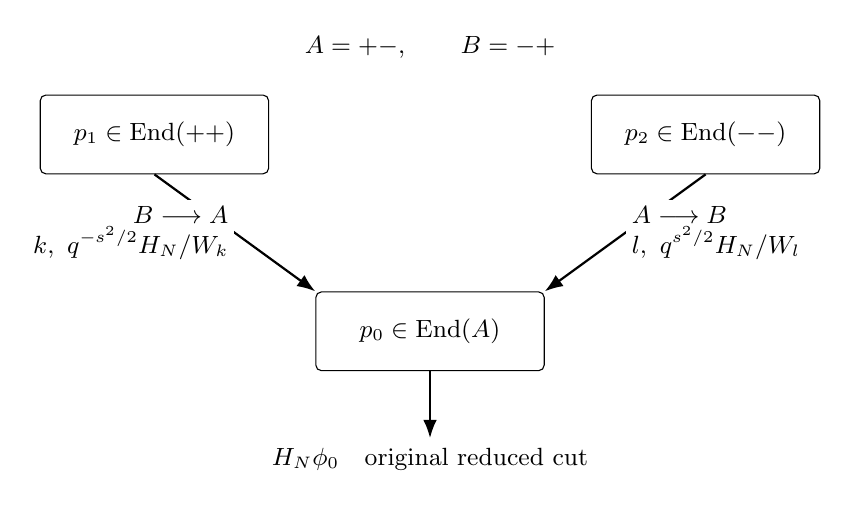
\begin{tikzpicture}[>=Latex,every node/.style={font=\small},
 coupon/.style={draw,rounded corners=2pt,minimum width=2.9cm,minimum height=1cm}]
\node[coupon] (p0) at (0,0) {$p_0\in\End(A)$};
\node[coupon] (p1) at (-3.5,2.5) {$p_1\in\End(++)$};
\node[coupon] (p2) at (3.5,2.5) {$p_2\in\End(--)$};
\draw[->,thick] (p1.south) -- node[left,align=right,fill=white,inner sep=2pt] {$B\longrightarrow A$\\$k,\ q^{-s^2/2}H_N/W_k$} (p0.north west);
\draw[->,thick] (p2.south) -- node[right,align=left,fill=white,inner sep=2pt] {$A\longrightarrow B$\\$l,\ q^{s^2/2}H_N/W_l$} (p0.north east);
\draw[->,thick] (p0.south) -- ++(0,-.85) node[below] {$H_N\phi_0\quad\text{original reduced cut}$};
\node at (0,3.6) {$A=+-,\qquad B=-+$};
\end{tikzpicture}

\caption{A three-vertex contraction with original types retained.
The turns of equal-color coupons $p_1,p_2$ are maps $B\to A$ and
$A\to B$; their ordered product and $p_0\in\End(A)$ close in
$\Acal_0$. Indices $k,l$ range over $0,\ldots,d$. Edge scalars
are $q^{-s^2/2}$ and $q^{s^2/2}$, respectively; the additional
factors are $H_N/W_k$ and $H_N/W_l$.}
\label{mt:tree-figure}
\end{figure}
For this example the full unframed value is
\[
 H_N\sum_{k,l=0}^d\frac{H_N}{W_k}\frac{H_N}{W_l}
       \phi_0(p_0e_ke_l)\phi_s(p_1e_k)\phi_{-s}(p_2e_l).
\]
Only the two turn phases cancel; all edge and vertex factors remain.
Identity coupons are allowed, so no valence or nonzero-exponent
condition has entered the result.

\section{The scalar ledger, including negative mixed words}
The preceding contraction already includes all physical scalars.
We isolate a useful scalar when equal-color chirps are separated
from their normalized values and mixed words use $r_0^n$. This is
an exact bookkeeping identity, not a relative estimate for the
whole invariant.

Equation~\eqref{mt:monodromy} gives the mixed generators:
\[
\begin{array}{c|cc}
 &\text{positive crossing}&\text{negative crossing}\\\hline
 \text{start }A&r_0&q^{s^2}r_0^{-1}\\
 \text{start }B&q^{-s^2}r_0&r_0^{-1}.
\end{array}
\]
Each generator swaps order, also for a negative crossing. For a
word of length $L$ and exponent $n$, the exponent of $q^{s^2}$
starting at $A$ is $(L-n)/2-\lfloor L/2\rfloor
=-\lfloor n/2\rfloor$; starting at $B$ uses the ceiling. Hence
\begin{equation}\label{mt:mixed-words}
 p_{n,A}=q^{-\lfloor n/2\rfloor s^2}r_0^n,\qquad
 p_{n,B}=q^{-\lceil n/2\rceil s^2}r_0^n,
 \quad n\in\mathbb Z.
\end{equation}
These are full quotient identities, including every normal.

Give every endomorphism space the grading $\chi=0$, and set
$\chi(\Hom(A,B))=1$, $\chi(\Hom(B,A))=-1$.
It adds under compatible products. Table~\ref{mt:types} says each
turn scalar is $q^{(\chi_{\rm out}-\chi_{\rm in})s^2/2}$.
Temporarily put $\widetilde f=q^{-\chi s^2/2}f$ in each type.
Products still multiply, turns lose precisely their scalar, and
the final endomorphism is unchanged. A mixed word has
$\chi=\delta(n)$ starting at $A$ and $-\delta(n)$ starting at $B$,
where $\delta(n)$ is Euclidean parity, including when $n<0$.
Both formulas \eqref{mt:mixed-words} then leave $q^{-ns^2/2}$.
For equal-color words the same scalar is
$C_{N,n}(s)/C_{N,n}(0)$ in \eqref{mt:angles}; their remaining
chirps are still evaluated at shifted angles.

\begin{proposition}[Exact quadratic scalar]\label{mt:scalar}
Let the actual checked-crossing powers in the original diagram be
$n_i$, and let $w(D)$ be its oriented writhe. Exclude the
index-dependent factors $H_N/W_k$, the single closing factor $H_N$,
and the shifted chirp or fixed $r_0^{n_i}$ at each box. The product
of the remaining scalar ratios is
\begin{equation}\label{mt:scalar-value}
 A_N(s)=q^{(-w(D)-\sum_i n_i)s^2/2}.
\end{equation}
For the positive checked-braid convention, put $o_i=1$ when the
original oriented strands in box $i$ are parallel, $o_i=-1$ when
antiparallel. Then $w(D)=\sum_i o_i n_i$ and the exponent integer
is $-2\sum_{o_i=1}n_i$.
\end{proposition}
\begin{proof}
The grading leaves $q^{-n_i s^2/2}$ from every box.
Equation~\eqref{mt:twist} adds $q^{-w(D)s^2/2}$.
Bending maps have already been counted in the turns, and their
snake identities leave no further monomial; the closure leaves
the one excluded $H_N$. Multiplying proves the formula.
Reversing one oriented crossing tangent reverses the writhe sign,
whereas reversing both preserves it, proving the final assertion.
\end{proof}
For example an exponent $-1$ word starting at $A$ has scalar
$q^{s^2}$ before the turn grading, whereas one starting at $B$
has scalar one. Neither conversion is counted twice. The ledger
does not say that a whole polynomial or invariant is its complete
value times $A_N(s)$: moving arguments and changed quotient
products remain inside the exact expression.

\section{Finite reproduction and interfaces}
The accompanying \texttt{check.py} compares physical module
matrices, finite crossing sums and explicit currying contractions
with these polynomial formulas in exact finite fields. Its report
lists all levels, rational meridian parameters and primes. It
checks both parities, collisions, negative powers, all six turns,
full pivotal moments, curls, moving ordinary circles and a small tree. These finite checks are
supplementary to the all-level coefficient and path proofs. Run
\[
 \texttt{python3 papers/meridian-tangles/check.py --output DIRECTORY}.
\]
Python and NumPy are required. The script rejects disabled
assertions and removes an old success record before checking.

The finite input to an analytic tree theorem is now explicit:
\eqref{mt:vertex} is its actual local tensor,
\eqref{mt:trace-grid} its full trace,
\eqref{mt:kernel-main} its edge kernel and
\eqref{mt:message} its original recursion. An asymptotic theorem
must estimate the whole contraction, including complementary
Newton indices and repeated-root normals. None of the identities
above establishes dominance of a selected saddle or positive
subcollection.

\begin{thebibliography}{9}
\bibitem{Newton} \emph{Newton coefficients and positive sources for Conway tangles},
companion paper, \href{https://sashakolpakov.github.io/murakamis_dream/papers/newton-tangles.pdf}{repository edition}.
\bibitem{Finite} \emph{Finite spectral evaluation and uniform filling bounds},
companion paper, \href{https://sashakolpakov.github.io/murakamis_dream/papers/filling-bounds.pdf}{repository edition}.
\bibitem{ADO} Y. Akutsu, T. Deguchi and T. Ohtsuki,
\emph{Invariants of colored links}, J. Knot Theory Ramifications
\textbf{1} (1992), 161--184,
\href{https://doi.org/10.1142/S0218216592000094}{doi:10.1142/S0218216592000094}.
\bibitem{CGP} F. Costantino, N. Geer and B. Patureau-Mirand,
\emph{Some remarks on the unrolled quantum group of $\mathfrak{sl}(2)$},
J. Pure Appl. Algebra \textbf{219} (2015), 3238--3262,
\href{https://arxiv.org/abs/1406.0410}{arXiv:1406.0410}.
\bibitem{GPT} N. Geer, B. Patureau-Mirand and V. Turaev,
\emph{Modified quantum dimensions and re-normalized link invariants},
Compositio Math. \textbf{145} (2009), 196--212,
\href{https://doi.org/10.1112/S0010437X08003795}{doi:10.1112/S0010437X08003795}.
\end{thebibliography}
\end{document}
